\documentclass[11pt]{article}
\usepackage{amsmath}
\usepackage{amssymb}
\usepackage[margin=1in]{geometry}
\usepackage{titling}
\usepackage{graphicx}
\usepackage{float}
\usepackage{booktabs}
\usepackage{xcolor}
\usepackage{hyperref}
\usepackage{tocloft}

\hypersetup{
    colorlinks=true,
    linkcolor=black,
    citecolor=black,
    urlcolor=black,
    pdftitle={Loss Functions as Noise Models},
}

\title{
  Loss Functions as Noise Models\\
  \vspace{15px}
  \Large Signal Detection and Estimation Theory, Project 3
}

\author{
  \Large Varun Shastry (2023112005)
  % add teammates here
}
\date{
    \today
}

\numberwithin{figure}{section}
\numberwithin{equation}{section}

\setlength{\cftsecnumwidth}{3em}
\setlength{\cftsubsecnumwidth}{3em}

\begin{document}

\maketitle

\tableofcontents
\clearpage

\section{Introduction}

\subsection{The problem}

When we fit a model to data, we pick a loss function and choose the parameters that make the
loss as small as possible. The two most common losses are the mean squared error (MSE) and the mean absolute error (MAE). The survey by Terven et al.~\cite{terven} gives rules for choosing between them, for example that MAE is better when the data has outliers. But it doesn't explain these rules using estimation theory.

Minimizing a loss is the same as maximising likelihood. So every loss assumes some
distribution for the noise. We later show in Section~\ref{sec:losses} we show that MSE assumes Gaussian noise and MAE assumes Laplace noise.

In this project we observe what happens when this assumption is wrong. For example, if we use MSE but the noise is actually Laplace, does the estimate still be correct on average? what about the variance? Intuitively we'd expect variance to be larger than that of the best possible estimator.

We measure this loss in accuracy using the Cram\'er--Rao lower bound (CRLB), which provides a lower bound for the variance of any unbiased estimator ~\cite{kay}. For our study, we find the ratio of the CRLB for the true noise, to the variance of our estimator,
\[
  \text{efficiency ratio} = \frac{\operatorname{Var}(\hat A)}{\text{CRLB}}.
\]
A ratio of 1 simply means the estimator is as good as possible. A ratio of 2 means its variance is twice the CRLB, hence it needs twice as many samples to be as accurate as the best estimator.

\subsection{The setup}

We start with the simplest case, which is estimating a DC level in noise, as in Kay. We observe $N$ samples
\begin{equation}
  x[n] = A + w[n], \qquad n = 0, 1, \dots, N-1,
  \label{eq:dc}
\end{equation}
where $A \in \mathbb{R}$ is the unknown constant and $w[n]$ is the noise. The noise samples $w[n]$ are i.i.d.\ with zero mean and an assumed density $p_w(w)$ that is symmetric about zero, so $p_w(-w) = p_w(w)$. We want to estimate the parameter $A$ from the samples.

Stacking the samples and the noise into vectors,
\[
  \mathbf{x} = [x[0], x[1], \dots, x[N-1]]^\top, \qquad
  \mathbf{w} = [w[0], w[1], \dots, w[N-1]]^\top,
\]
the model becomes
\[
  \mathbf{x} = A\mathbf{1} + \mathbf{w},
\]
where $\mathbf{1} = [1, 1, \dots, 1]^\top$ is the column vector of $N$ ones. This is a special case of linear regression, $\mathbf{y} = \mathbf{X}\boldsymbol{\theta} + \mathbf{w}$, with $\mathbf{X} = \mathbf{1}$ and $\boldsymbol{\theta} = A$. Here $\mathbf{X}^\top\mathbf{X} = \mathbf{1}^\top\mathbf{1} = N$, so the $1/N$ in our results becomes
$(\mathbf{X}^\top\mathbf{X})^{-1}$ for the general regression model, which we study later.

\section{Losses as noise assumptions}
\label{sec:losses}

In this section we derive the MSE and MAE losses. In both cases we write the likelihood of the samples for an assumed noise distribution and find the $A$ that maximises it.

From \eqref{eq:dc}, $w[n] = x[n] - A$, so each sample $x[n]$ has density $p_w(x[n]-A)$. The
samples are i.i.d., so the likelihood is the product of these densities,
\begin{equation}
  p(\mathbf{x}; A) = \prod_{n=0}^{N-1} p_w(x[n]-A).
  \label{eq:lik}
\end{equation}
The maximum likelihood estimator (MLE) is the value of $A$ that makes this as large as possible
for the observed samples. It is easier to work with the log of the likelihood. Since the log is an increasing function, the maximum is at the same $A$, so
\[
  \hat A = \arg\max_A \, p(\mathbf{x}; A) = \arg\max_A \, \ln p(\mathbf{x}; A)
  = \arg\max_A \sum_{n=0}^{N-1} \ln p_w(x[n]-A).
\]

\subsection{Gaussian noise gives squared error}

Let the noise be Gaussian with zero mean and variance $\sigma^2$,
\[
  w[n] \overset{\text{i.i.d.}}{\sim} \mathcal{N}(0, \sigma^2), \qquad
  p_w(w) = \frac{1}{\sqrt{2\pi\sigma^2}} \exp\!\left(-\frac{w^2}{2\sigma^2}\right).
\]
Then $x[n] \sim \mathcal{N}(A, \sigma^2)$, and from \eqref{eq:lik} the likelihood is
\begin{align*}
  p(\mathbf{x}; A) &= \prod_{n=0}^{N-1} \frac{1}{\sqrt{2\pi\sigma^2}}
  \exp\!\left(-\frac{(x[n]-A)^2}{2\sigma^2}\right) \\
  &= \frac{1}{(2\pi\sigma^2)^{N/2}}
  \exp\!\left(-\frac{1}{2\sigma^2}\sum_{n=0}^{N-1}(x[n]-A)^2\right).
\end{align*}
Taking the log gives
\[
  \ln p(\mathbf{x}; A) = -\frac{N}{2}\ln(2\pi\sigma^2)
  - \frac{1}{2\sigma^2}\sum_{n=0}^{N-1}(x[n]-A)^2 .
\]
The first term does not depend on $A$. The second term has a minus sign, so maximising
$\ln p(\mathbf{x}; A)$ is the same as minimising
\[
  J(A) = \sum_{n=0}^{N-1}(x[n]-A)^2 .
\]
This is the squared error loss. So minimising MSE is the same as finding the MLE under Gaussian
noise.

Setting the derivative of $J$ to zero,
\begin{align*}
  \frac{dJ}{dA} = -2\sum_{n=0}^{N-1}(x[n]-A) &= 0 \\
  \sum_{n=0}^{N-1} x[n] - NA &= 0 .
\end{align*}
We thus obtain
\[
  \boxed{\hat A = \frac{1}{N}\sum_{n=0}^{N-1} x[n] = \bar{x}}
\]
So under Gaussian noise, the MLE of $A$ is the sample mean.

\subsection{Laplace noise gives absolute error}

Now let the noise be Laplace with zero mean and a scale parameter $b > 0$,
\[
  w[n] \overset{\text{i.i.d.}}{\sim} \operatorname{Laplace}(0, b), \qquad
  p_w(w) = \frac{1}{2b}\exp\!\left(-\frac{|w|}{b}\right).
\]
This density is also symmetric about zero, but its tails are heavier because the Gaussian density falls off like $e^{-w^2}$, while the Laplace density only falls off like $e^{-|w|}$. So large noise
values are more likely with Laplace noise, thus the data might tend to have a few samples far away from the rest.

We follow the same steps as in the Gaussian case. From \eqref{eq:lik} the likelihood is
\begin{align*}
  p(\mathbf{x}; A) &= \prod_{n=0}^{N-1} \frac{1}{2b}
  \exp\!\left(-\frac{|x[n]-A|}{b}\right) \\
  &= \frac{1}{(2b)^N}
  \exp\!\left(-\frac{1}{b}\sum_{n=0}^{N-1}|x[n]-A|\right),
\end{align*}
and its log is
\[
  \ln p(\mathbf{x}; A) = -N\ln(2b) - \frac{1}{b}\sum_{n=0}^{N-1}|x[n]-A| .
\]
Again the first term does not depend on $A$, so maximising $\ln p(\mathbf{x}; A)$ is the same as
minimising
\[
  J(A) = \sum_{n=0}^{N-1}|x[n]-A| .
\]
This is the absolute error loss. So minimising MAE is the same as finding the MLE under Laplace noise.

Here we cannot just set the derivative to zero, because $|x[n]-A|$ has a sharp edge at $A = x[n]$ where its non-differentiable. Everywhere else the derivative is
\[
  \frac{dJ}{dA} = -\sum_{n=0}^{N-1}\operatorname{sign}(x[n]-A),
\]
Hence, each sample above $A$ adds $-1$ and each sample below $A$ adds $+1$. So the derivative is the number of samples below
$A$ minus the number of samples above $A$.

If more samples lie above $A$ than below it, the derivative is negative and $J$ decreases as $A$
increases. Once more samples lie below $A$, the derivative is positive and $J$ increases. As $A$
moves from left to right it passes the samples one by one, so the derivative goes up in steps,
from $-N$ to $+N$. So $J$ is smallest where the derivative changes sign, which is where half the
samples lie on each side of $A$. For odd $N$ the derivative never equals zero. It jumps from $-1$
to $+1$ at the middle sample, so the minimum is at this corner of $J$, which is the sample median,
\[
  \boxed{\hat A = \operatorname{median}\bigl(x[0], x[1], \dots, x[N-1]\bigr)}
\]
For example, with the samples $1$, $2$ and $10$, the derivative is $-3, -1, +1, +3$ as $A$ passes
each sample, so $J$ is smallest at $A = 2$. Thus, under Laplace noise, the MLE of $A$ is the sample median. 

To summarise, MSE assumes Gaussian noise and gives the mean, and MAE assumes Laplace noise and gives the median!

\section{The Cram\'er--Rao lower bound}
\label{sec:crlb}

The CRLB gives a lower bound on the variance of any unbiased estimator of $A$. From
Kay~\cite[Theorem 3.1]{kay}, if the likelihood satisfies the regularity condition
\[
  E\!\left[\frac{\partial \ln p(\mathbf{x}; A)}{\partial A}\right] = 0 \quad \text{for all } A,
\]
then every unbiased estimator $\hat A$ satisfies
\begin{equation}
  \operatorname{Var}(\hat A) \geq \frac{1}{I(A)}, \qquad
  I(A) = E\!\left[\left(\frac{\partial \ln p(\mathbf{x}; A)}{\partial A}\right)^{2}\right],
  \label{eq:crlb}
\end{equation}
where $I(A)$ is the Fisher information. When $\ln p(\mathbf{x}; A)$ is twice differentiable, the
Fisher information can also be written as
\begin{equation}
  I(A) = -E\!\left[\frac{\partial^2 \ln p(\mathbf{x}; A)}{\partial A^2}\right].
  \label{eq:fisher2}
\end{equation}

From \eqref{eq:lik}, the log-likelihood is a sum over the samples, so its derivative is also a
sum,
\[
  \frac{\partial \ln p(\mathbf{x}; A)}{\partial A} = \sum_{n=0}^{N-1} s(x[n]; A), \qquad
  s(x; A) = \frac{\partial}{\partial A} \ln p_w(x - A).
\]
Each term $s(x[n]; A)$ depends on only one sample, so the terms are independent, and each has
zero mean by the regularity condition. The variance of a sum of independent zero-mean terms is
the sum of their variances, so
\begin{equation}
  I(A) = E\!\left[\Bigl(\sum_{n=0}^{N-1} s(x[n]; A)\Bigr)^{2}\right]
  = \sum_{n=0}^{N-1} E\!\left[s(x[n]; A)^2\right] = N\, i(A), \qquad
  i(A) = E\!\left[s(x; A)^2\right].
  \label{eq:fisher-iid}
\end{equation}
So we only need $i(A)$, the Fisher information of a single sample.

\subsection{CRLB for Gaussian noise}

For Gaussian noise,
\[
  \ln p_w(x - A) = -\frac{1}{2}\ln(2\pi\sigma^2) - \frac{(x-A)^2}{2\sigma^2}.
\]
Differentiating with respect to $A$,
\[
  s(x; A) = \frac{x - A}{\sigma^2} = \frac{w}{\sigma^2}.
\]
So the information in one sample is
\[
  i(A) = \frac{E[w^2]}{\sigma^4} = \frac{\sigma^2}{\sigma^4} = \frac{1}{\sigma^2}.
\]
The second form also \eqref{eq:fisher2} gives the same answer, since
$\partial^2 \ln p_w(x-A)/\partial A^2 = -1/\sigma^2$ for every $x$. Thus using the i.i.d additivity property of Fisher information,
$I(A) = N/\sigma^2$, and we obtain
\[
  \boxed{\text{CRLB}_{\text{Gauss}} = \frac{\sigma^2}{N}}
\]

\subsection{CRLB for Laplace noise}

For Laplace noise,
\[
  \ln p_w(x - A) = -\ln(2b) - \frac{|x - A|}{b}.
\]
For $x \neq A$, the derivative with respect to $A$ is
\[
  s(x; A) = \frac{\operatorname{sign}(x - A)}{b} = \frac{\operatorname{sign}(w)}{b}.
\]
The sign is either $+1$ or $-1$, so $s(x; A)^2 = 1/b^2$ for every sample. Then
\[
  i(A) = E\!\left[\frac{1}{b^2}\right] = \frac{1}{b^2},
\]
so $I(A) = N/b^2$, and we thus obtain
\[
  \boxed{\text{CRLB}_{\text{Laplace}} = \frac{b^2}{N}}
\]

The regularity condition holds, because the Laplace density is symmetric and so
\[
  E[s(x; A)] = \frac{1}{b}\bigl(P(w > 0) - P(w < 0)\bigr) = \frac{1}{b}\left(\frac{1}{2} - \frac{1}{2}\right) = 0.
\]
The derivative does not exist at $x = A$, but this single point has probability zero, so it does
not change any of the expectations.

Note that we could only use the first form \eqref{eq:crlb} of Fisher information here. The second derivative of $|x - A|$ is zero everywhere except at $x = A$, so the second form
\eqref{eq:fisher2} would give $i(A) = 0$ and an infinite bound, which is wrong! As mentioned above, the second form needs $\ln p_w$ to be twice differentiable, and it's not the case here with the Laplacian noise!
\newline
Kay~\cite{kay} also states that an unbiased estimator reaches the CRLB only if we can write an expression of the type:
\[
  \frac{\partial \ln p(\mathbf{x}; A)}{\partial A} = I(A)\bigl(g(\mathbf{x}) - A\bigr)
\]
for some function $g$. Under Gaussian noise this holds with $g(\mathbf{x}) = \bar x$. Under Laplace noise the derivative is $\frac{1}{b}\sum_n \operatorname{sign}(x[n] - A)$, which is a
step function of $A$ and cannot be written in this form. So for a fixed $N$, no unbiased estimator reaches the Laplace
bound exactly. In Section~\ref{sec:median} we see that the median reaches it as $N$ grows!

\section{Estimators under the wrong noise}
\label{sec:mismatch}

We now find the variance of the sample mean and the sample median under both noise types, and
compare each with the CRLB from Section~\ref{sec:crlb}.

\subsection{The sample mean}

The sample mean is unbiased for any noise with zero mean,
\[
  E[\bar x] = \frac{1}{N}\sum_{n=0}^{N-1} E\bigl[A + w[n]\bigr] = A.
\]
The samples are independent, so
\begin{equation}
  \operatorname{Var}(\bar x) = \frac{1}{N^2}\sum_{n=0}^{N-1}\operatorname{Var}(w[n])
  = \frac{\operatorname{Var}(w)}{N}.
  \label{eq:varmean}
\end{equation}
This only uses the variance of the noise so far, without considering the shape of a distribution.
\subsubsection{Under Gaussian Noise}
Under Gaussian noise, $\operatorname{Var}(w) = \sigma^2$, so $\operatorname{Var}(\bar x) =
\sigma^2/N$. This equals the CRLB, so the sample mean is efficient under Gaussian noise.

\subsubsection{Under Laplacian Noise}

Under Laplace noise, the noise has zero mean, so $\operatorname{Var}(w) = E[w^2] - (E[w])^2
= E[w^2]$. Writing out the expectation,
\[
  E[w^2] = \int_{-\infty}^{\infty} w^2 \, \frac{1}{2b} e^{-|w|/b} \, dw .
\]
\[
  E[w^2] = 2 \cdot \frac{1}{2b}\int_{0}^{\infty} w^2 e^{-w/b} \, dw
  = \frac{1}{b}\int_{0}^{\infty} w^2 e^{-w/b} \, dw .
\]
We find the integral using integration by parts twice. Let
\[
  I_k = \int_{0}^{\infty} w^k e^{-w/b} \, dw .
\]
Using integration by parts: 
\[
  \int_0^\infty u \, dv = \Bigl[uv\Bigr]_0^\infty - \int_0^\infty v \, du .
\]
For $I_2$ we take $u = w^2$ and $dv = e^{-w/b}\,dw$, so $du = 2w\,dw$ and $v = -b\,e^{-w/b}$.
Then
\begin{align*}
  I_2 &= \Bigl[-b\,w^2 e^{-w/b}\Bigr]_0^\infty + 2b\int_0^\infty w\, e^{-w/b}\,dw \\
      &= 0 + 2b\, I_1 .
\end{align*}
The boundary term is zero, because at $w = 0$ the factor $w^2$ is zero, and as $w \to \infty$ the exponential $e^{-w/b}$ goes to zero faster than $w^2$ grows. In the same way, for $I_1$ we
take $u = w$ and $dv = e^{-w/b}\,dw$,
\begin{align*}
  I_1 &= \Bigl[-b\,w\, e^{-w/b}\Bigr]_0^\infty + b\int_0^\infty e^{-w/b}\,dw \\
      &= 0 + b\Bigl[-b\, e^{-w/b}\Bigr]_0^\infty \\
      &= b \cdot b = b^2 .
\end{align*}
Putting these together, $I_2 = 2b \cdot b^2 = 2b^3$, and so
\begin{align*}
  \operatorname{Var}(w) = E[w^2] &= \frac{1}{b}\, I_2 \\
  &= 2b^2 .
\end{align*}
Now from \eqref{eq:varmean},
\[
  \boxed{\operatorname{Var}(\bar x)_{\text{Laplace}} = \frac{2b^2}{N} = 2 \times \text{CRLB}_{\text{Laplace}}}
\]
This holds for every $N$, not only for large $N$! The mean is still correct on average, but its variance is twice the CRLB, so it needs twice as many samples to be as accurate as the best estimator! The intuitive reason is that every sample gets the same weight $1/N$, including the few large samples that Laplace noise produces, and these pull the mean away from $A$.

\subsection{The sample median}
\label{sec:median}

The noise is symmetric about zero, so the samples are symmetric about $A$, and so is the distribution of the median. So the median is also unbiased. Its exact variance has no simple formula, but for large $N$ the sample median is approximately Gaussian with
variance~\cite[Ch.~21]{vdv}
\begin{equation}
  \operatorname{Var}(\operatorname{median}) \approx \frac{1}{4N\, p_w(0)^2}.
  \label{eq:varmedian}
\end{equation}
The median only depends on which samples lie above and below $A$, so its accuracy depends on
how many samples fall close to $A$. This is set by the height of the noise density at the centre,
$p_w(0)$. A taller peak puts more samples near $A$ and gives a more accurate median.

For Laplace noise, $p_w(0) = 1/(2b)$, so from \eqref{eq:varmedian}
\[
  \boxed{\operatorname{Var}(\operatorname{median})_{\text{Laplace}} \approx
  \frac{1}{4N \cdot \frac{1}{4b^2}} = \frac{b^2}{N} = \text{CRLB}_{\text{Laplace}}}
\]
So for large $N$ the median reaches the CRLB under Laplace noise. It is asymptotically efficient.

For Gaussian noise, $p_w(0) = 1/\sqrt{2\pi\sigma^2}$, so
\[
  \boxed{\operatorname{Var}(\operatorname{median})_{\text{Gauss}} \approx
  \frac{1}{4N \cdot \frac{1}{2\pi\sigma^2}} = \frac{\pi}{2}\cdot\frac{\sigma^2}{N}
  \approx 1.57 \times \text{CRLB}_{\text{Gauss}}}
\]
Under Gaussian noise, the distance of each sample from $A$ carries information. The median
throws this away, since it only looks at the order of the samples, and this costs about $57\%$
more variance than the mean.

\subsection{Predicted efficiency ratios}

Dividing each variance by the CRLB for the true noise gives the efficiency ratios in
Table~\ref{tab:predicted}.

\begin{table}[H]
\centering
\begin{tabular}{lcc}
\toprule
Estimator (loss) & Gaussian noise & Laplace noise \\
\midrule
Sample mean (MSE)   & $1$ & $2$ \\
Sample median (MAE) & $\pi/2 \approx 1.57$ & $1$ \\
\bottomrule
\end{tabular}
\caption{Predicted efficiency ratio $\operatorname{Var}(\hat A)/\text{CRLB}$ for each estimator
and each true noise.}
\label{tab:predicted}
\end{table}

Each estimator is efficient under the noise it assumes and loses efficiency under the other one.
The values for the mean are exact for every $N$, while the values for the median hold only for
large $N$. We check these values by Monte Carlo simulation in Section~\ref{sec:sims}.

\section{Simulation results}
\label{sec:sims}

In this section we check the results of Section~\ref{sec:mismatch} by simulation, and then look
at two noise types where the theory so far does not directly apply. All the code is in the
\texttt{sim/} folder of the project, with one script per simulation.

Every simulation follows the same Monte Carlo method. We fix the true value $A = 1$ and repeat
the experiment $R = 5000$ times. In each trial we draw $N$ fresh noise samples, form
$x[n] = A + w[n]$, and compute both the sample mean and the sample median. This gives $5000$
values of each estimator. Their average estimates $E[\hat A]$, and their sample variance
estimates $\operatorname{Var}(\hat A)$. Dividing the variance by the CRLB gives the measured
efficiency ratio.

Since we only use $5000$ trials, the measured variance is itself a little noisy. For estimates that
are roughly Gaussian, the relative error of a sample variance computed from $R$ values is about
$\sqrt{2/R}$, which is $2\%$ here. So a measured ratio of $0.97$ is in agreement with a predicted
ratio of $1$.

\subsection{Gaussian and Laplace noise}
\label{sec:simA}

We first check the predicted ratios of Table~\ref{tab:predicted}. We use $\sigma = 1$ for the
Gaussian noise and $b = 1$ for the Laplace noise. The ratios do not depend on these values, since
both the variances and the CRLBs scale in the same way. The code is in
\texttt{sim/sim\_A\_mean\_vs\_median.py}.

Table~\ref{tab:simA} shows the measured ratios at $N = 100$ next to the predicted ones. All four
agree with the theory. The mean has ratio $1$ under Gaussian noise and $2$ under Laplace noise,
and the median has ratio close to $\pi/2$ under Gaussian noise.

\begin{table}[H]
\centering
\begin{tabular}{lcccc}
\toprule
 & \multicolumn{2}{c}{Gaussian noise} & \multicolumn{2}{c}{Laplace noise} \\
Estimator & Predicted & Measured & Predicted & Measured \\
\midrule
Sample mean (MSE)   & $1$    & $0.968$ & $2$ & $2.007$ \\
Sample median (MAE) & $1.571$ & $1.512$ & $1$ & $1.169$ \\
\bottomrule
\end{tabular}
\caption{Predicted and measured efficiency ratio $\operatorname{Var}(\hat A)/\text{CRLB}$ at
$N = 100$, from $5000$ trials.}
\label{tab:simA}
\end{table}

The only value that is clearly away from its prediction is the median under Laplace noise,
$1.169$ instead of $1$. This is expected, because \eqref{eq:varmedian} only holds for large $N$.
To see this, we repeat the experiment for $N$ from $10$ to $1000$. Figure~\ref{fig:simA} shows
the result.

\begin{figure}[H]
\centering
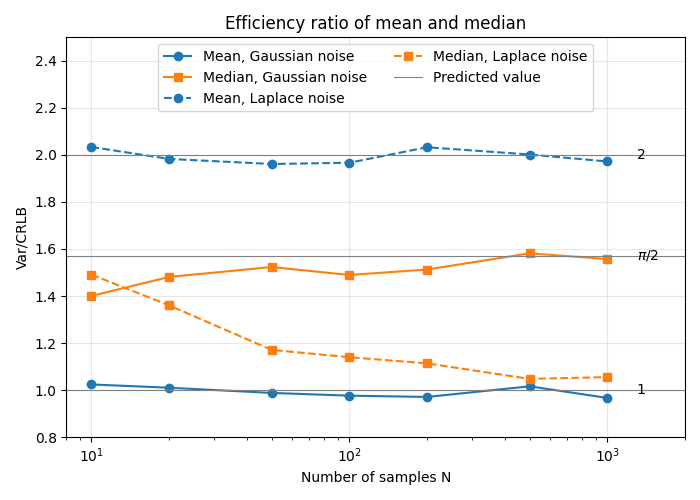
\includegraphics[width=0.8\linewidth]{../figures/simA_ratio_vs_N.png}
\caption{Measured efficiency ratio against the number of samples $N$. The grey lines are the
predicted values $1$, $\pi/2$ and $2$.}
\label{fig:simA}
\end{figure}

We can observe two different behaviours in Figure~\ref{fig:simA}. The two curves for the mean are
flat, at $1$ for Gaussian noise and $2$ for Laplace noise, already from $N = 10$. This matches
Section~\ref{sec:mismatch}, where we found $\operatorname{Var}(\bar x) = \operatorname{Var}(w)/N$
exactly for every $N$. The two curves for the median change with $N$. Under Laplace noise the
ratio starts at about $1.5$ for $N = 10$ and slowly comes down towards $1$, reaching $1.05$ at
$N = 1000$. Under Gaussian noise it starts at $1.4$ and rises towards $\pi/2$. So the median
only becomes efficient under Laplace noise once $N$ is large, while the mean is twice as bad as
the best estimator at every $N$.

\clearpage
\addcontentsline{toc}{section}{References}
\begin{thebibliography}{9}
\bibitem{kay} S.~M.~Kay, \emph{Fundamentals of Statistical Signal Processing, Volume I,
  Estimation Theory}, Prentice Hall, 1993.
\bibitem{terven} J.~Terven, D.~M.~Cordova-Esparza, J.~A.~Romero-Gonz\'alez, A.~Ram\'irez-Pedraza
  and E.~A.~Ch\'avez-Urbiola, ``A comprehensive survey of loss functions and metrics in deep
  learning,'' \emph{Artificial Intelligence Review}, vol.~58, article 195, 2025.
\bibitem{vdv} A.~W.~van der Vaart, \emph{Asymptotic Statistics}, Cambridge University Press,
  1998.
\end{thebibliography}

\end{document}
